\section{Interactive Advertising Bureau (IAB)}
The predefined category set should be well-defined and fit for the purposes of the task. Since the focus of this project is improving advertising, the predefined category set should be a category set useful for advertising. 


%The machine learning need a predefined set of categories for the clustering. It is already mentioned that Wikipedia has articles stored under categories and that the categories form a tree or graph structure. The problem is that there are too many categories that are not relevant for our categorization.

%The problem is therefore using IAB's categories for the clustering. 

IAB is a business organization that develops, researches and maintains industry standards for the online advertising industry. The organization works for creating, coalescing and maintaining standards and practices in online advertising. In addition, IAB researches and shares knowledge on the advertisement, and IAB members are responsible for distributing 86 \% of all the online advertisement in the US \cite{IABabout}.

IAB provides different guidelines for advertising, including \emph{Quality Assurance Guidelines Taxonomy} (QAGT). This taxonomy is a well-defined for advertising, and can be viewed as a category set. The set is split into two \emph{layers} also called \emph{tiers}. The layers are created for varying the grade of speciality between the first tier (a general or broad level) and the second tier (a deepening level). The first tier contains a total of 23 categories, examples are \emph{Business} and \emph{Food \& Drinks}. The second tier contains 371 subcategories, where each subcategory is a more specific category of a category in the first tier. 

%, where the categories are subcategories of a category in the first tier.
Figure \ref{fig:IAB} shows the taxonomy of IAB as defined on their web page where the first tier is all the category names written in white (e.g., \emph{Food \& Drinks}) and the second tier is followed under the first tier (e.g., \emph{American Cuisine}). 

We wanted to use IAB's taxonomy as our output category set, i.e., the keywords are mapped to one or more categories in the category set. 


\begin{figure}[t]
\begin{subfigure}{\textwidth}
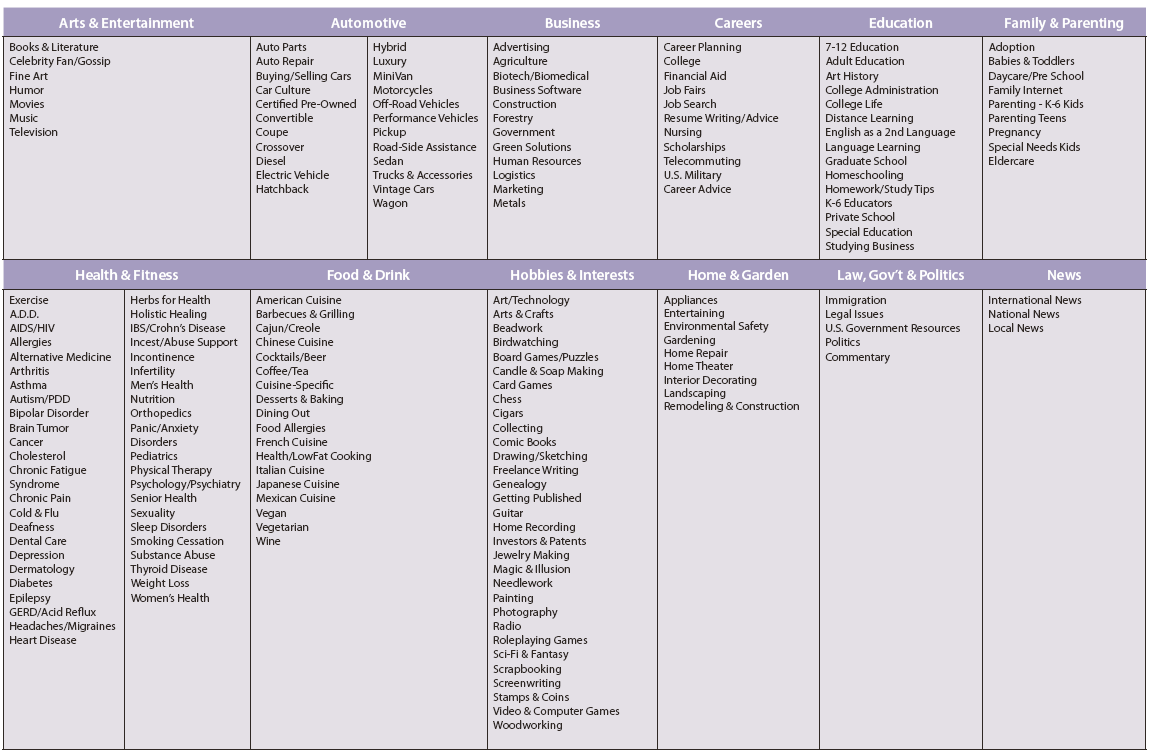
\includegraphics[width=\textwidth]{Chapters/Background/Taxonomy-1.png}
\end{subfigure}
\begin{subfigure}{\textwidth}
\centering
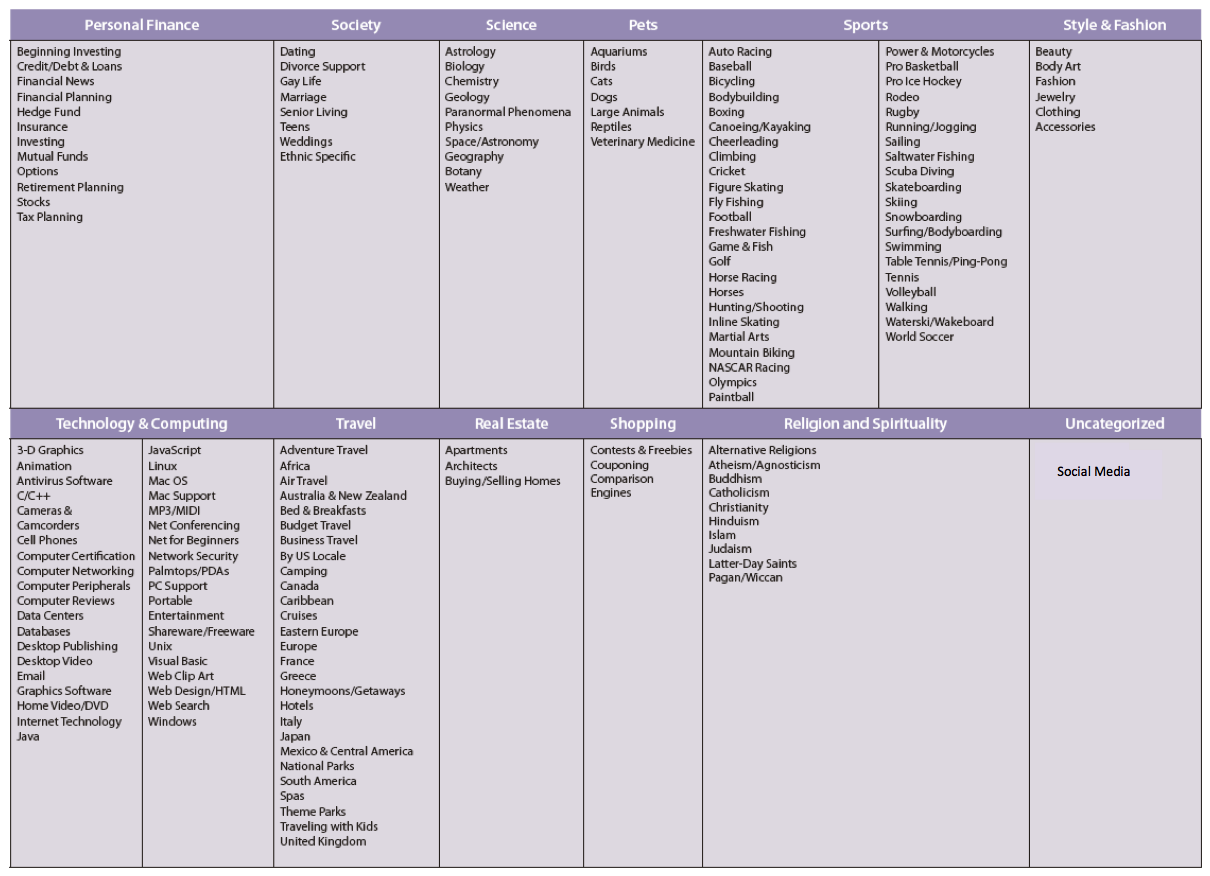
\includegraphics[width=\textwidth]{Chapters/Background/Taxonomy-2.png}
\end{subfigure}
\caption{Categories of the IAB Taxonomy}
\label{fig:IAB}
\end{figure}